
%	PACKAGES AND THEMES
%----------------------------------------------------------------------------------------

\documentclass{beamer}

\mode<presentation> {

\usetheme{default}

\usetheme{Madrid}

\usecolortheme{whale}
}
\usepackage{float}
\usepackage{graphicx}
\usepackage{caption}
\usepackage{subcaption}
\usepackage{graphicx} % Allows including images
\usepackage{booktabs} % Allows the use of \toprule, \midrule and \bottomrule in tables
%\usepackage{hyperref}
\usepackage{listings}
\lstset{
%language=C,
frame=single, 
breaklines=true,
columns=fullflexible
}
\usepackage{subcaption}
\usepackage{url}
\usepackage{authblk}
\usepackage{tikz}
\usetikzlibrary{arrows.meta,positioning}
\usepackage{pgfplots}
\pgfplotsset{compat=1.17}
\usepackage{tkz-fct}
\usepackage{mathrsfs}
\usepackage{txfonts}
\usepackage{tkz-euclide} 
\usetikzlibrary{calc,math}
\usepackage{float}
\newcommand\norm[1]{\left\lVert#1\right\rVert}
\renewcommand{\vec}[1]{\mathbf{#1}}
\providecommand{\pr}[1]{\ensuremath{\Pr\left(#1\right)}}
\usepackage[export]{adjustbox}
\usepackage[utf8]{inputenc}
\usepackage{amsmath}
\newcommand{\myvec}[1]{\ensuremath{\begin{pmatrix}#1\end{pmatrix}}}
\title[Wireless channel]{Modelling and performance analysis of $wireless$ $channel$ using $Probability$} 


\setbeamertemplate{caption}[numbered]
\begin{document}
\author{ANNU}
%\includegraphics[height=1cm,width=2cm]{iith.png} % Your name
\institute[ANNU,IIT HYDERABAD] % Your institution as it will appear on the bottom of every slide, may be shorthand to save space
{\textbf{PROJECT PRESENTATION-AI5002}\\
\\
BY-\textbf{ANNU} (EE21RESCH01010)\\
INDIAN INSTITIUTE OF TECHNOLOGY , HYDERABAD \\ % Your institution for the title page
\medskip
\textit{ee21resch01010@iith.ac.in} % Your email address
}
\date{\today} % Date, can be changed to a custom date

\logo{
  \includegraphics[height=1cm]{iith.png}
}

\begin{frame}
\titlepage % Print the title page as the first slide
\end{frame}

\begin{frame}
\frametitle{Overview} % Table of contents slide, comment this block out to remove it
\tableofcontents % Throughout your presentation, if you choose to use \section{} and \subsection{} commands, these will automatically be printed on this slide as an overview of your presentation
\end{frame}


\section{Probability Concepts} % Sections can be created in order to organize your presentation into discrete blocks, all sections and subsections are automatically printed in the table of contents as an overview of the talk
%------------------------------------------------

\subsection{Probability application in Communication} % A subsection can be created just before a set of slides with a common theme to further break down your presentation into chunks
\section{Wireless Communication Model}
\subsection{Noise Channel Model}
\section{Fading}
\subsection{Types of fading}
\section{Gaussian Noise}
\section{Rayleigh Fading Simulation}
\section{Performance Analysis of wireless channels}
\section{Performance Analysis of Communication System}
\subsection{Outage Probability}
\subsection{Error Rate}
\section{Digital Communication Model}
\section{Conclusion}
\begin{frame}{ABSTRACT}
\begin{block}{}
\begin{enumerate}
    \item Modelling of wireless channels is done in general fading conditions and their performance is  analysed using 2 parameters-
    \begin{enumerate}
        \item Outage Probability
        \item Bit Error Rate
    \end{enumerate}
    \item Fading in wireless channel is very important like Rayleigh fading for channel estimation and it is simulated in this presentation.\\
\end{enumerate}

\end{block}
\begin{figure}
        \centering
        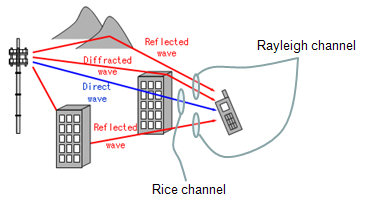
\includegraphics[width=0.4\columnwidth]{wireless_chanel.png}
        \caption{Wireless channel}
    \end{figure}
\end{frame}


%%%%%%%%%%%%%%%%%%%%%%%%%%%%%%%%%%%%%%%%%%%%%%%%%%%%%%%%%%



\frame
{
  \frametitle{Q-Function}

  \begin{itemize}
   \item \textit{Q function} is a convenient way to express right-tail probabilities for Gaussian random variables
   \item Mathematically, this can be expressed as:
   \begin{eqnarray}
    Q(x)&=1-F_X(x)=1-P(X\le{x})\\
    &=P(X>x)=\frac{1}{\sqrt{2\pi}}\int\limits_{x}^{\infty}e^{-t^2/2}dt
   \end{eqnarray}
  \end{itemize}

  }


%%%%%%%%%%%%%%%%%%%%%%%%%%%%%%%%%%%%%%%%%%%%%%%%%%%%%%%%%%

\frame
{
  \frametitle{Where Does Randomness in Wireless communication Occur?}

  \begin{itemize}
   \item Several locations where randomness occurs in the communications system includes:
   \begin{itemize}
    \item Transmission channel
    \item Data generation at information source
    \item Clock jitter
    \item Processing latency
    \item No guiding medium between transmitter and receiver.\\
    \item Multiple signals superpose at the receiver. As a result of destructive interference, strength of signal fades(weakens). This effect is known as fading.
    \item $\ldots$
   \end{itemize}

  \end{itemize}


  }
%%%%%%%%%%%%%%%%%%%%%%%%%%%%%%%%%%%%%%%%%%%%%%%%%%%%%%%%%%

\frame
{
  \frametitle{Noise Channel Model}
  
  \centering
  Binary Information Source $\rightarrow$ $m[n]$\\
  $\downarrow$\\
  Transmitter $\rightarrow$ $s(t)$\\
  $\downarrow$\\
  Channel $\rightarrow$ $s(t)+n(t)$\\
  $\downarrow$\\
  Receiver $\leftarrow$ $r(t)$\\
  $\downarrow$\\
  Binary Information Sink $\leftarrow$ $\hat{m}[n]$

}




%%%%%%%%%%%%%%%%%%%%%%%%%%%%%%%%%%%%%%%%%%%%%%%%%%%%%%%%%%

\frame
{
  \frametitle{Gaussian Random Variable}
  
  \begin{itemize}
   \item We frequently use \textbf{Gaussian random variables} to model noise contribution to transmitted signal
   \item Gaussian random variable mathematically expressed as:
   \begin{equation}
    f(x)=\frac{1}{\sqrt{2\pi{\sigma^2}}}e^{-((x-\mu)/\sigma)^2/2}
   \end{equation}
   where $\mu$ is the mean and $\sigma$ is the standard deviation
  \end{itemize}

  
}




%%%%%%%%%%%%%%%%%%%%%%%%%%%%%%%%%%%%%%%%%%%%%%%%%%%%%%%%%%
\begin{frame}{AWGN}

\begin{block}{}
\begin{itemize}
    \item \textbf{Additive}\\ It is because it is added to any noise that might be intrinsic to the information system.
    \item \textbf{White}\\ It refers to the idea that the noise has the same power distribution at every frequency.
    \item \textbf{Gaussian}\\It is because it has a normal distribution with mean of 0 as time domain average value sums to 0.

\end{itemize}
\end{block}
\begin{figure}
    \centering
    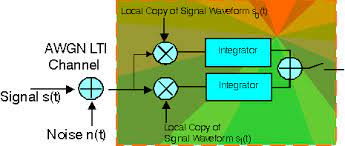
\includegraphics[width=0.5\columnwidth]{agn_sum.jpg}
    \caption{AWGN CHANNEL}
    \label{fig:1}
\end{figure}

\end{frame}

\begin{frame}{Gaussian Noise Simulation}

\begin{figure}[H]
	\centering
	\begin{subfigure}{.3\textwidth}
	    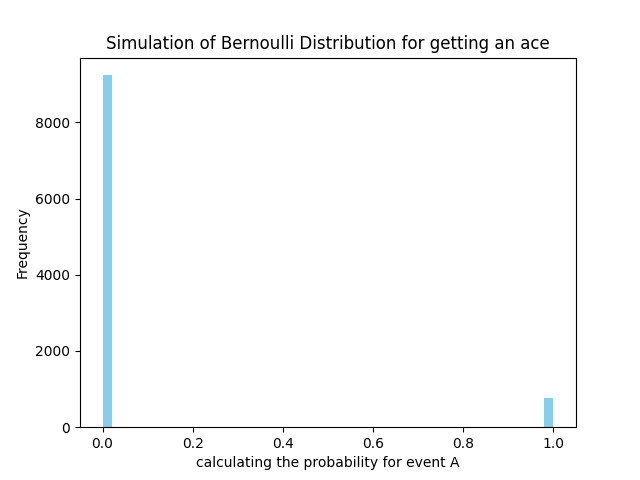
\includegraphics[width=\textwidth]{Figure_1.png}
		\caption{Gaussian Noise in time domain}
	\end{subfigure}
	\begin{subfigure}{.3\textwidth}
		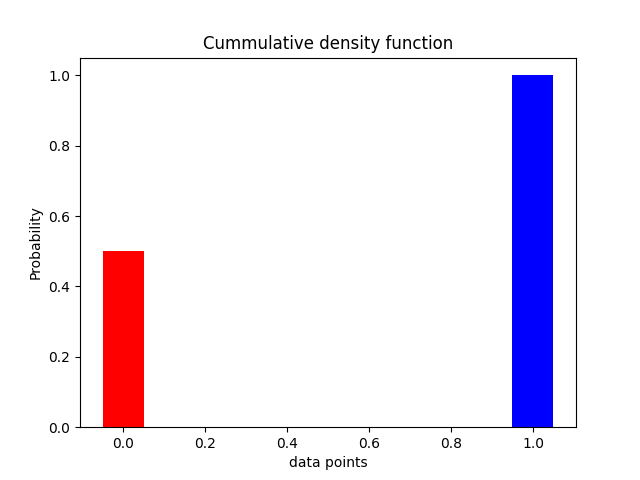
\includegraphics[width=\textwidth]{Figure_2.png}
		\caption{Gaussian Noise in frequency domain}
	\end{subfigure}
	\begin{subfigure}{.3\textwidth}
		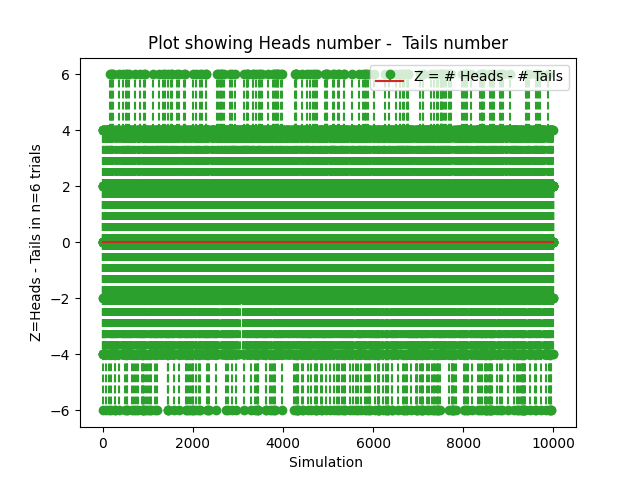
\includegraphics[width=\textwidth]{Figure_3.png}
		\caption{Complex Gaussian Noise in time domain}
	\end{subfigure}
		\begin{subfigure}{.3\textwidth}
		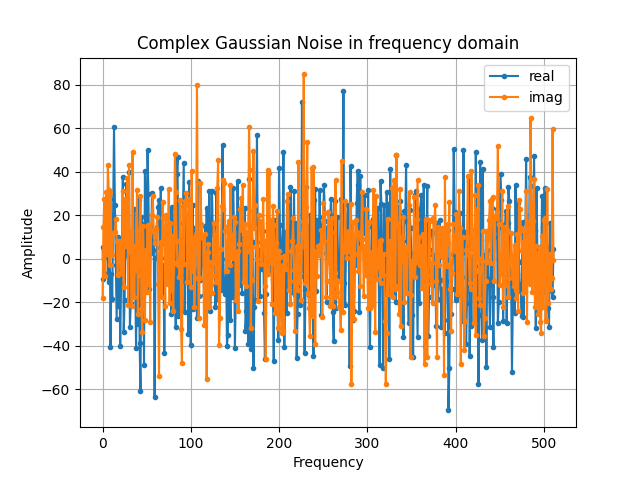
\includegraphics[width=\textwidth]{Figure_4.png}
		\caption{Complex Gaussian Noise in frequency domain}
	\end{subfigure}
	\caption{ Gaussian Noise Simulation }
\end{figure}
\end{frame}

\frame
{
  \frametitle{Bivariate Gaussian}

General definition for bivariate
Gaussian density with parameters $\mu_X$, $\mu_Y$, $\sigma_X^2$,
$\sigma_Y^2$, and correlation coefficient $\rho$ is given by:
\begin{equation}
f_{XY}(x,y)=\frac{\exp\left(\frac{-1}{2(1-\rho^2)}\left(\left(\frac{x-\mu_X}{\sigma_X}\right)^2-2\rho\left(\frac{x-\mu_X}{\sigma_X}\right)\left(\frac{y-\mu_Y}{\sigma_Y}\right)+\left(\frac{y-\mu_Y}{\sigma_Y}\right)^2\right)\right)}{2\pi\sigma_X\sigma_Y\sqrt{1-\rho^2}},
\end{equation}
where {\it correlation coefficient} is defined as:
\begin{equation}
    \rho=E\left[\left(\frac{x-\mu_X}{\sigma_X}\right)\left(\frac{y-\mu_Y}{\sigma_Y}\right)\right].
\end{equation}
}
  
\frame{
\frametitle{AWGN Channel Simulation}
\begin{figure}[H]
	\centering
	\begin{subfigure}{.4\textwidth}
		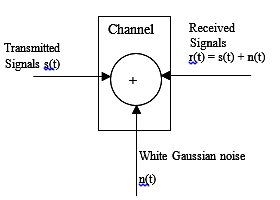
\includegraphics[width=\textwidth]{awgn.png}
		\caption{AWGN CHANNEL}
	\end{subfigure}
	\begin{subfigure}{.5\textwidth}
		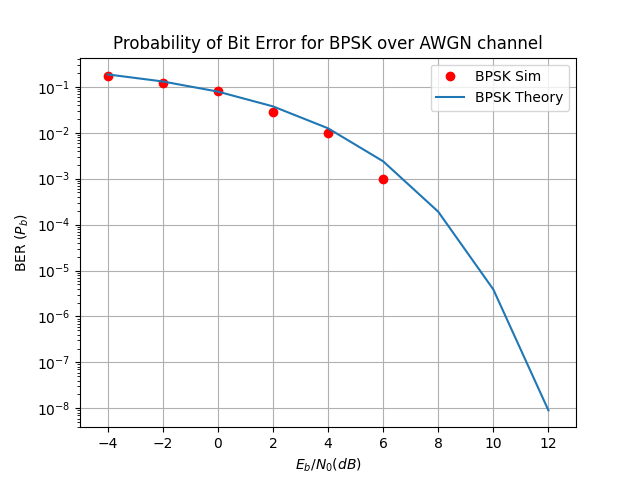
\includegraphics[width=\textwidth]{ber_bpsk.png}
		\caption{BER versus SNR(Db) for BPSK with \textbf{AWGN}}
	\end{subfigure}
\end{figure}
}
%%%%%%%%%%%%%%%%%%%%%%%%%%%%%%%%%%%%%%%%%%%%%%%%%%%%%%%%%%

\frame
{
  \frametitle{Multipath Fading in wireless communication}
  \begin{itemize}
      \item \textbf{Multipath fading:}A propagation phenomenon that results in signals reaching the receiver by two or more paths, which we experience in real-world wireless systems
      \begin{figure}
       \centering
       \includegraphics[width=0.4\columnwidth]{mul1.jpg}
       \caption{Multipath fading}
       \label{multipath}
       \end{figure}
       
       \begin{figure}
       \centering
       \includegraphics[width=0.4\columnwidth]{mul2.jpg}
       \caption{Multipath fading}
       \label{multipath}
       \end{figure}
  \end{itemize}
}
  
 \frame{
   \frametitle{Types of Fading}
   There are two types of fading from a time domain perspective
   \begin{itemize}
       \item \textbf{Slow Fading} 
       \item \textbf{Fast Fading}
   \end{itemize}
   There are two types of fading from a frequency domain perspective
   \begin{itemize}
       \item \textbf{ Frequency Selective Fading}
       \item \textbf{Flat Fading}
   \end{itemize}
   }
  

\frame{
\frametitle{Illustration of fading}
\begin{enumerate}
    \item In the figure 7 given below, the red shape shows our signal in the frequency domain
    \item black curvy line shows the current channel condition over frequency.
    \item Because the narrower signal is experiencing the same channel conditions throughout the whole signal, it’s experiencing \textbf{flat fading}. 
    \item The wider signal is very much experiencing frequency \textbf{selective fading}.
\end{enumerate}
       \begin{figure}
       \centering
       \includegraphics[width=0.7\columnwidth]{flat_sel.png}
       \caption{Multipath fading}
       \label{7}
       \end{figure}}
\frame{
\begin{enumerate}
    \item Here is an example of a 16 MHz wide signal that is continuously transmitting.
    \item There are several moments in the middle where there’s a period of time a piece of signal is missing. 
    \item This example depicts frequency selective fading, which causes holes in the signal that wipe out some frequencies but not others.
\end{enumerate} 
        \begin{figure}
       \centering
       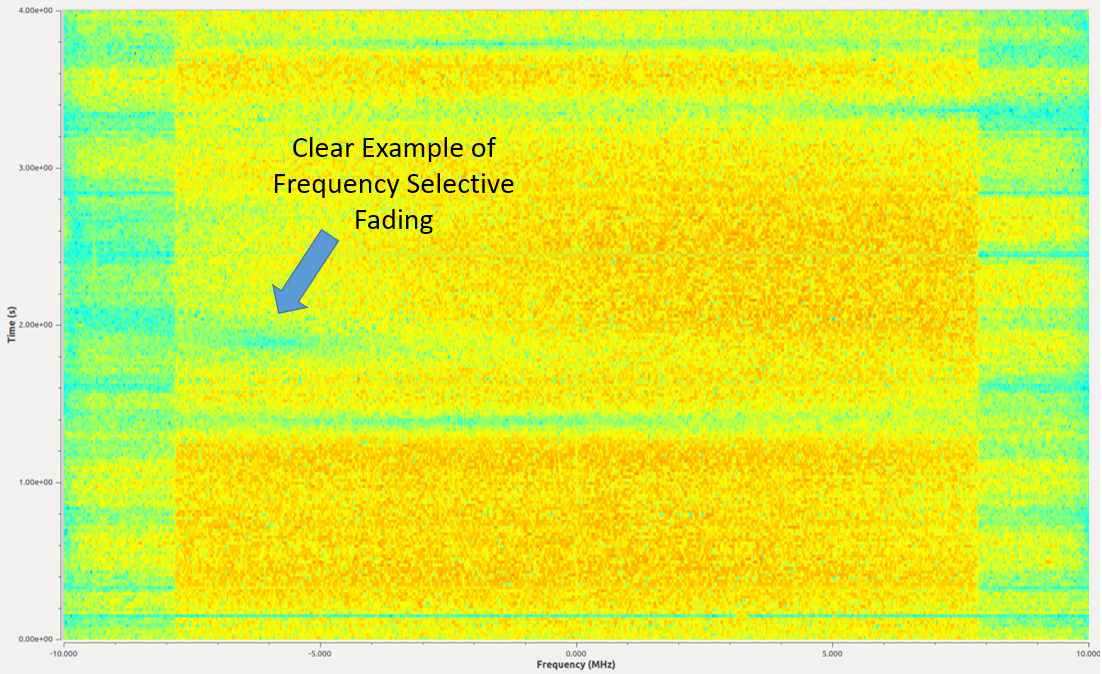
\includegraphics[width=0.5\columnwidth]{fading_example.png}
       \caption{Multipath fading}
       \label{fading_example}
       \end{figure}

}
%%%%%%%%%%%%%%%%%%%%%%%%%%%%%%%%%%%%%%%%%%%%%%%%%%%%%%%%%%
\begin{frame}{Rayleigh Distribution}
\begin{block}{PDF of Rayleigh}
 The probability density function of the Rayleigh distribution is
\begin{align}
    { f(x;\sigma )={\frac {x}{\sigma ^{2}}}e^{-x^{2}/(2\sigma ^{2})},\quad x\geq 0,}  
\end{align}
where  $\sigma$ is the scale parameter of the distribution.
\end{block}

\end{frame}
\begin{frame}{Rayleigh Channel simulation}
    \begin{figure}
    \centering
    \includegraphics[width=\columnwidth]{rayleigh.jpg}
    \caption{Rayleigh Fading}
    \label{4}
\end{figure}   
\end{frame}
\begin{frame}{Rayleigh fading Channel Modelling}
The fading channel coefficient h depends on factors 
\begin{enumerate}
    \item attenuation ($a_i$)
    \item time delay($\tau_i$)
\end{enumerate}
\begin{block}{Modelling the distribution of the fading channel coefficient}
\begin{align}
    h&=\sum_{i=0}^{L-1}a_i\exp{(-j2\pi f_c \tau_i)}\\
    &=\sum_{i=0}^{L-1}a_i\cos{(2\pi f_c \tau_i)}-j\sum_{i=0}^{L-1}a_i\sin{(2\pi f_c \tau_i)}\\
    &=X+jY
\end{align}
where X=$\sum_{i=0}^{L-1}a_i\cos{(2\pi f_c \tau_i)}$ and Y=$-\sum_{i=0}^{L-1}a_i\sin{(2\pi f_c \tau_i)}$
\end{block}
\end{frame}
\begin{frame}{}
\begin{block}{Joint Pdf of X and Y}
\begin{align}
&X,Y\sim \mathcal{N}(\mu ,\sigma^2)\\
f_X(x)=&\frac{1}{\sqrt{2\pi \sigma^2}}exp{\frac{-(x-\mu)^2}{2\sigma^2}}\\
f_Y(y)=&\frac{1}{\sqrt{2\pi \sigma^2}}exp{\frac{-(y-\mu)^2}{2\sigma^2}}
\end{align}
Assuming X and Y are independent random variables and substituting $\mu=0$ for simplification 
\begin{align}
f_{XY}(x,y)=&\frac{1}{{2\pi \sigma^2 }}exp{\left(-(x^2+y^2)\right)}  \label{eq1} 
\end{align}
\end{block}
\end{frame}
\begin{frame}{}

\begin{block}{ Distribution of the fading channel in terms of its Amplitude and phase using Jacobian }
\begin{align}
&h=x+jy=ae^{j\phi}\\
&a=\sqrt{x^2+y^2}, \phi=\tan^{-1}{\frac{y}{x}}\label{eq2}\\
&f_{A,{\Phi}}(a,\phi)=f_{XY}(x,y)\big{|}J_{XY}\big{|}\\
&\big{|}J_{XY}\big{|} =
\begin{vmatrix}
\frac{\partial x}{\partial a} & \frac{\partial y}{\partial a} \\
\frac{\partial x}{\partial \phi} & \frac{\partial y}{\partial \phi} 
\end{vmatrix}=\begin{vmatrix}
\cos{\phi} & \sin{\phi} \\
-a\sin{\phi} & a\cos{\phi} 
\end{vmatrix}\label{eq3}
\end{align}
from \eqref{eq1},\eqref{eq2} and \eqref{eq3} we get
\begin{align}
  &f_{A,{\Phi}}(a,\phi)= \frac{a}{{2\pi \sigma^2}}\exp{\left(\frac{-a^2}{2\sigma^2}\right)} 
\end{align}
\end{block}
\end{frame}
\begin{frame}{}
 \begin{block}{Marginal distribution of A}
 \begin{align}
   f_A(a)&=\int_{-\pi}^{\pi}f_{A,{\Phi}}(a,\phi)\;d\phi\\
   &= \int_{-\pi}^{\pi}\frac{a}{{2\pi \sigma^2}}\exp{\left(\frac{-a^2}{2\sigma^2}\right)}\;d\phi\\
   &=\frac{a}{\sigma^2}\exp{\left(\frac{-a^2}{2\sigma^2}\right)}
 \end{align}
 \end{block}
 \begin{enumerate}
     \item The coefficient follows the Rayleigh distribution and is fading in nature.
     \item  It is therefore called as a Rayleigh fading channel.
 \end{enumerate}
\end{frame}


%%%%%%%%%%%%%%%%%%%%%%%%%%%%%%%%%%%%%%%%%%%%%%%%%%%%%%%%%%
\frame{
\frametitle{Performace Analysis of wireless channels}

\begin{block}{\textbf{Outage Probability}}
Outage probability can be easily computed if we know the probability distribution characteristics of the fading.
\begin{math}
P_{out}(R)=Pr((log(1+|h|^2 \times SNR) <R)
\end{math}
\end{block}
\begin{block}{Error rate}
In digital transmission, the number of bit errors is the number of received bits of a data stream over a communication channel that have been altered due to noise, interference, distortion or bit synchronization errors. The bit error rate (BER) is the number of bit errors per unit time.

\end{block}}

\frame{
\frametitle{Simulation Results-Outage Probability}
\begin{figure}
    \centering
    \includegraphics[width=0.6\columnwidth]{outage_prob.png}
    \caption{Outage probability of MRC processing in Rayleigh fading channel}
    \label{5}
\end{figure}

}

\frame{
\frametitle{Simulation Results-Error Rate}
\begin{figure}
    \centering
    \includegraphics[width=0.6\columnwidth]{symbol.png}
    \caption{Symbol error rate Vs EbN0 for QPSK over i.i.d Rayleigh flat fading channel with MRC processing at the receiver}
    \label{6}
\end{figure}
}



\begin{frame}[fragile]{Einstein-Wiener-Khinchin Theorem}

    \begin{itemize}
        \item In particular, we are interested in the {\it power spectral density} (PSD) of a signal, which is related to the autocorrelation function via the {\it Einstein-Wiener-Khintchine} (EWK) Relations:
            \begin{equation}
                  S_X(f)=\int_{-\infty}^{\infty}R_X(\tau)e^{-j2\pi{f}{\tau}}d\tau
            \end{equation}
            \begin{equation}                 
                  R_X(\tau)=\int_{-\infty}^{\infty}S_X(f)e^{j2\pi{f}{\tau}}df
            \end{equation} 
        \item Relating the PSD between input $x(t)$ and output $y(t)$ of a system $h(t)$, we have the following very important result:
            \begin{equation}
                  S_Y(f)=|H(f)|^2S_X(f)
            \end{equation}                
    \end{itemize}
\end{frame}


\begin{frame}[fragile]{PSD Example}

  \begin{itemize}
    \item Find $S_X(f)$ of the following random process:
    \begin{equation}
        x(t)=A\cos(2\pi{f_c}t+\Theta),\nonumber
    \end{equation}
    where $\Theta$ is uniformly distributed over the interval $[-\pi,\pi]$.
    \item First solve for $R_X(\tau)$ by using:
    \begin{equation}
        R_X(\tau)=E\{x(t+\tau)x(t)\}=\frac{1}{2}A^2\cos(2\pi{f_c}\tau)\nonumber
    \end{equation}
    \item Then solve for the PSD using EWK relations:
    \begin{equation}
    \begin{split}
        S_X(f)&=\int_{-\infty}^{\infty}R_X(\tau)e^{-j2\pi{f}\tau}d\tau=\int_{-\infty}^{\infty}\frac{1}{2}A^2\cos(2\pi{f_c}\tau)e^{-j2\pi{f}\tau}d\tau\\
        &=\int_{-\infty}^{\infty}\frac{1}{4}A^2\left(e^{j2\pi{f_c}\tau}+e^{-j2\pi{f_c}\tau}\right)e^{-j2\pi{f}\tau}d\tau\\
        &=\frac{A^2}{4}(\delta(f-f_c)+\delta(f+f_c))\nonumber
    \end{split}
    \end{equation}
  \end{itemize}
  
\end{frame}


%%%%%%%%%%%%%%%%%%%%%%%%%%%%%%%%%%%%%%%%%%%%%%%%%%%%%%%%%%

\frame
{
  \frametitle{Anatomy of a Typical Digital Communication System}

\begin{figure}
    \centering
    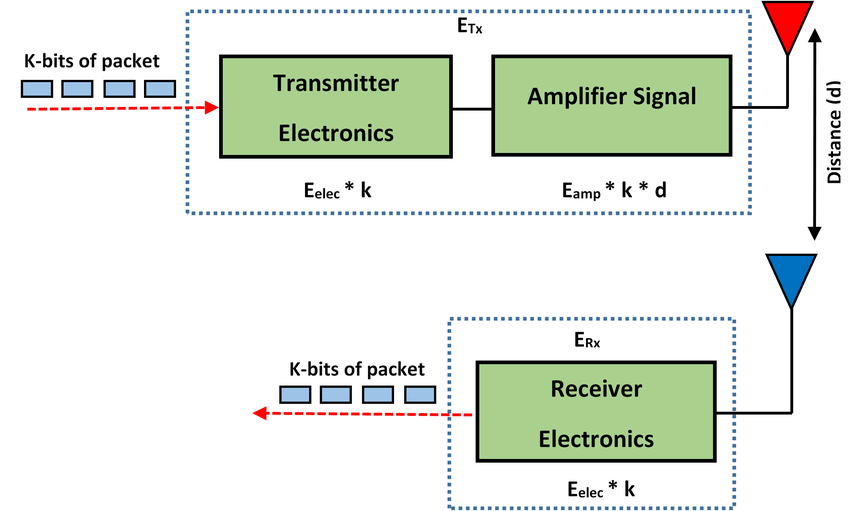
\includegraphics[width=0.7\columnwidth]{wireless_model.png}
    \caption{Digital Communication System Block Diagram}
    \label{8}
\end{figure}
}

\frame
{
  \frametitle{Shannon's Channel Capacity}
  \begin{equation}
    C=B\log_{2}(1+SNR)\qquad\mathsf{[b/s]}
  \end{equation}
  \begin{figure}
      \centering
      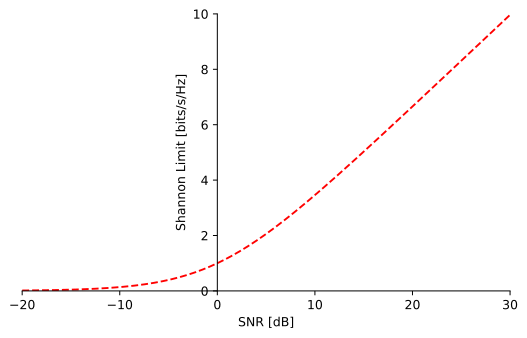
\includegraphics[width=0.5\columnwidth]{shannon_limit.png}
      \caption{Shannan limit $\frac{C}{B}$ versus SNR }
      \label{}
  \end{figure}
}

\frame
{
  \frametitle{Filtered AWGN Channel}

  \begin{itemize}
    \item We know that the power spectral density of white Gaussian noise is equal to:
    \begin{equation}
        S_N(f)=\mathbb{F}\{R_n(\tau)\}=\int\limits_{-\infty}^{\infty}R_n(\tau)e^{-j2\pi{f}\tau}d\tau=\frac{N_0}{2}
    \end{equation}
    \item When this noise is passed through an LTI system with impulse response $h(t)$, the output power spectral density will be defined by the Einstein-Wiener-Khinchin (EWK) Theorem, namely:
    \begin{equation}
        S_Y(f)=|H(f)|^2S_N(f)
    \end{equation}
  \end{itemize}

}

%%%%%%%%%%%%%%%%%%%%%%%%%%%%%%%%%%%%%%%%%%%%%%%%%%%%%%%%%%


\frame
{
  \frametitle{Average Bit Energy}

  \begin{itemize}
  \item The symbol energy is then $E_{s}$=$E_{-s}$=$A^2T$=$\frac{A^2}{R_b}$
    \begin{itemize}
        \item Notice how $E_{s}$ decreases as $R_{b}$ increases
    \end{itemize}
  \item We define the energy per bit as:
  \begin{equation}
    \bar{E}_{b}=P(1)\cdot\int_{-\infty}^{\infty}s_{1}^2(t)dt+P(0)\cdot\int_{-\infty}^{\infty}s_{2}^2(t)dt
  \end{equation}
  where $P(1)$ is the probability that the bit is a ``1'', and $P(0)$ is the probability that the bit is a ``0''
  \item Suppose $s_{1}(t)=s(t)$ and $s_{2}(t)=-s(t)$, then:
  \begin{equation}
    \bar{E}_{b}=E_{s}\{P(1)+P(0)\}=E_{s}=\int_{-\infty}^{\infty}s^2(t)dt=A^2T
  \end{equation}
  \end{itemize}

}




\frame
{
  \frametitle{Signal Vectors}

    \begin{itemize}
        \item Let $\phi_j(t)$ be an orthnormal set of functions on the time interval $[0,T]$ such that:
        \begin{equation}
            \int\limits_0^T\phi_i(t)\phi_j(t)dt=\left\{
            \begin{array}{ll}
              1 & i=j \\
              0 & \mathsf{otherwise}
            \end{array}
            \right.\nonumber
        \end{equation}
        \item Let $s_i(t)$ be the modulation signal that we can represent in terms of the orthonormal functions:
        \begin{equation}
            s_i(t)=\sum\limits_{k=1}^{N}s_{ik}\phi_k(t)
        \end{equation}
        which can be represented by the vector:
        \begin{equation}
            s_i(t)\rightarrow\mathbf{s}_i=(s_{i1},~s_{i2},~s_{i3},\ldots{s_{iN}})
        \end{equation}
    \end{itemize}

}

\frame
{
  \frametitle{Vector Manipulations}

    \begin{itemize}
        \item To find $s_{ik}$, solve:
        \begin{equation}
            \int\limits_0^Ts_i(t)\phi_l(t)dt=\sum\limits_{k=1}^{N}s_{ik}\int\limits_0^T\phi_k(t)\phi_l(t)dt=s_{il}
        \end{equation}
        \item The vector dot product between $s_i(t)$ and $s_j(t)$ is equal to:
        \begin{equation}
            \int\limits_0^Ts_i(t)s_j(t)dt=\mathbf{s}_i\cdot\mathbf{s}_j=\rho_{ij}
        \end{equation}
        while the energy of a signal $s_i(t)$ is equal to:
        \begin{equation}
            E_{s_i}=\int\limits_0^Ts_i^2(t)dt=\mathbf{s}_i\cdot\mathbf{s}_i=||\mathbf{s}_i||^2
        \end{equation}
    \end{itemize}
}
\frame
{
  \frametitle{Euclidean Distance}

    \begin{itemize}
        \item To compute the {\it Euclidean Distance} using signal space vectors, we need to solve:
        \begin{equation}
        \begin{split}
            d_{\min}^2&=\int\limits_0^T\Delta{s_{ij}^2(t)}dt=\int\limits_0^T(s_i(t)-s_j(t))^2dt\\
            &=||\mathbf{s}_i-\mathbf{s}_j||^2=(\mathbf{s}_i-\mathbf{s}_j)\cdot(\mathbf{s}_i-\mathbf{s}_j)\\
            &=E_{s_i}+E_{s_j}-2\rho_{ij}\nonumber
        \end{split}
        \end{equation}
        where:
        \begin{equation}
            \rho_{ij}=\int\limits_0^Ts_i(t)s_j(t)dt=\mathbf{s}_i\cdot\mathbf{s}_j
        \end{equation}
    \end{itemize}
}
\frame
{
  \frametitle{Solving for the Power Efficiency}

    \begin{itemize}
        \item Choose orthonormal basis functions $\phi_i(t)$, $i=1,2,\ldots,k$, where $k$ is the dimension of the signal space
        \item Find $\mathbf{s}_i$, $i=1,2,\ldots,M$ where $\mathbf{s}_i=(s_{i1},~s_{i2},\ldots{s_{ik}})$ and $s_{ij}=\int\limits_0^Ts_i(t)\phi_j(t)dt$
        \item Consequently, solve for:
        \begin{equation}
        \begin{split}
            d_{\min}^2&=\min\limits_{i\neq{j}}||{\mathbf{s}_i-\mathbf{s}_j}||^2\\
            \bar{E}_s&=\frac{1}{M}\sum\limits_{i=1}^{M}||\mathbf{s}_i||^2\\
            \bar{E}_b&=\bar{E}_s/\log_2(M)\\
            \varepsilon_p&=d_{\min}^2/\bar{E}_b\nonumber
        \end{split}
        \end{equation}
    \end{itemize}
}

\frame{
\frametitle{Conclusion}
\begin{enumerate}
    \item This paper presentation has considered wireless communication in a general fading environment, which can be reduced to other types of fading environments like Rayleigh.
    \item Rayleigh fading channel is simulated
    \item Obtained closed-form expressions for PDF and CDF of SNR for the interference-limited system case.
    \item  Some of the performance measures are evaluated and discussed in the presentation.
    \item Generalisation of communication system is analysed.
\end{enumerate}
 
}

\begin{frame}
\frametitle{Reference}
\footnotesize{
\begin{thebibliography}{99} % Beamer does not support BibTeX so references must be inserted manually as below

\newblock IEEE paper on Modelling and performance analysis of Wireless channel
\newblock Performance analysis of wireless communication system in general fading environment subjected to shadowing and interference
\end{thebibliography}
}

\end{frame}

%------------------------------------------------

\begin{frame}
\Huge{\centerline{THANK YOU.......}}
\end{frame}

%----------------------------------------------------------------------------------------

\end{document}